\subsubsection{Message Call}
\label{sec:message-call}
The message call is the mean to invoke a contract code and can be either
triggered by a transaction or by the execution of a contract. A message call
takes as input a state and the message itself (the data field) and returns an
output, that is from the point of view of Ethereum only relevant if the message
call is triggered by an execution.

\begin{figure}
	\begin{center}
		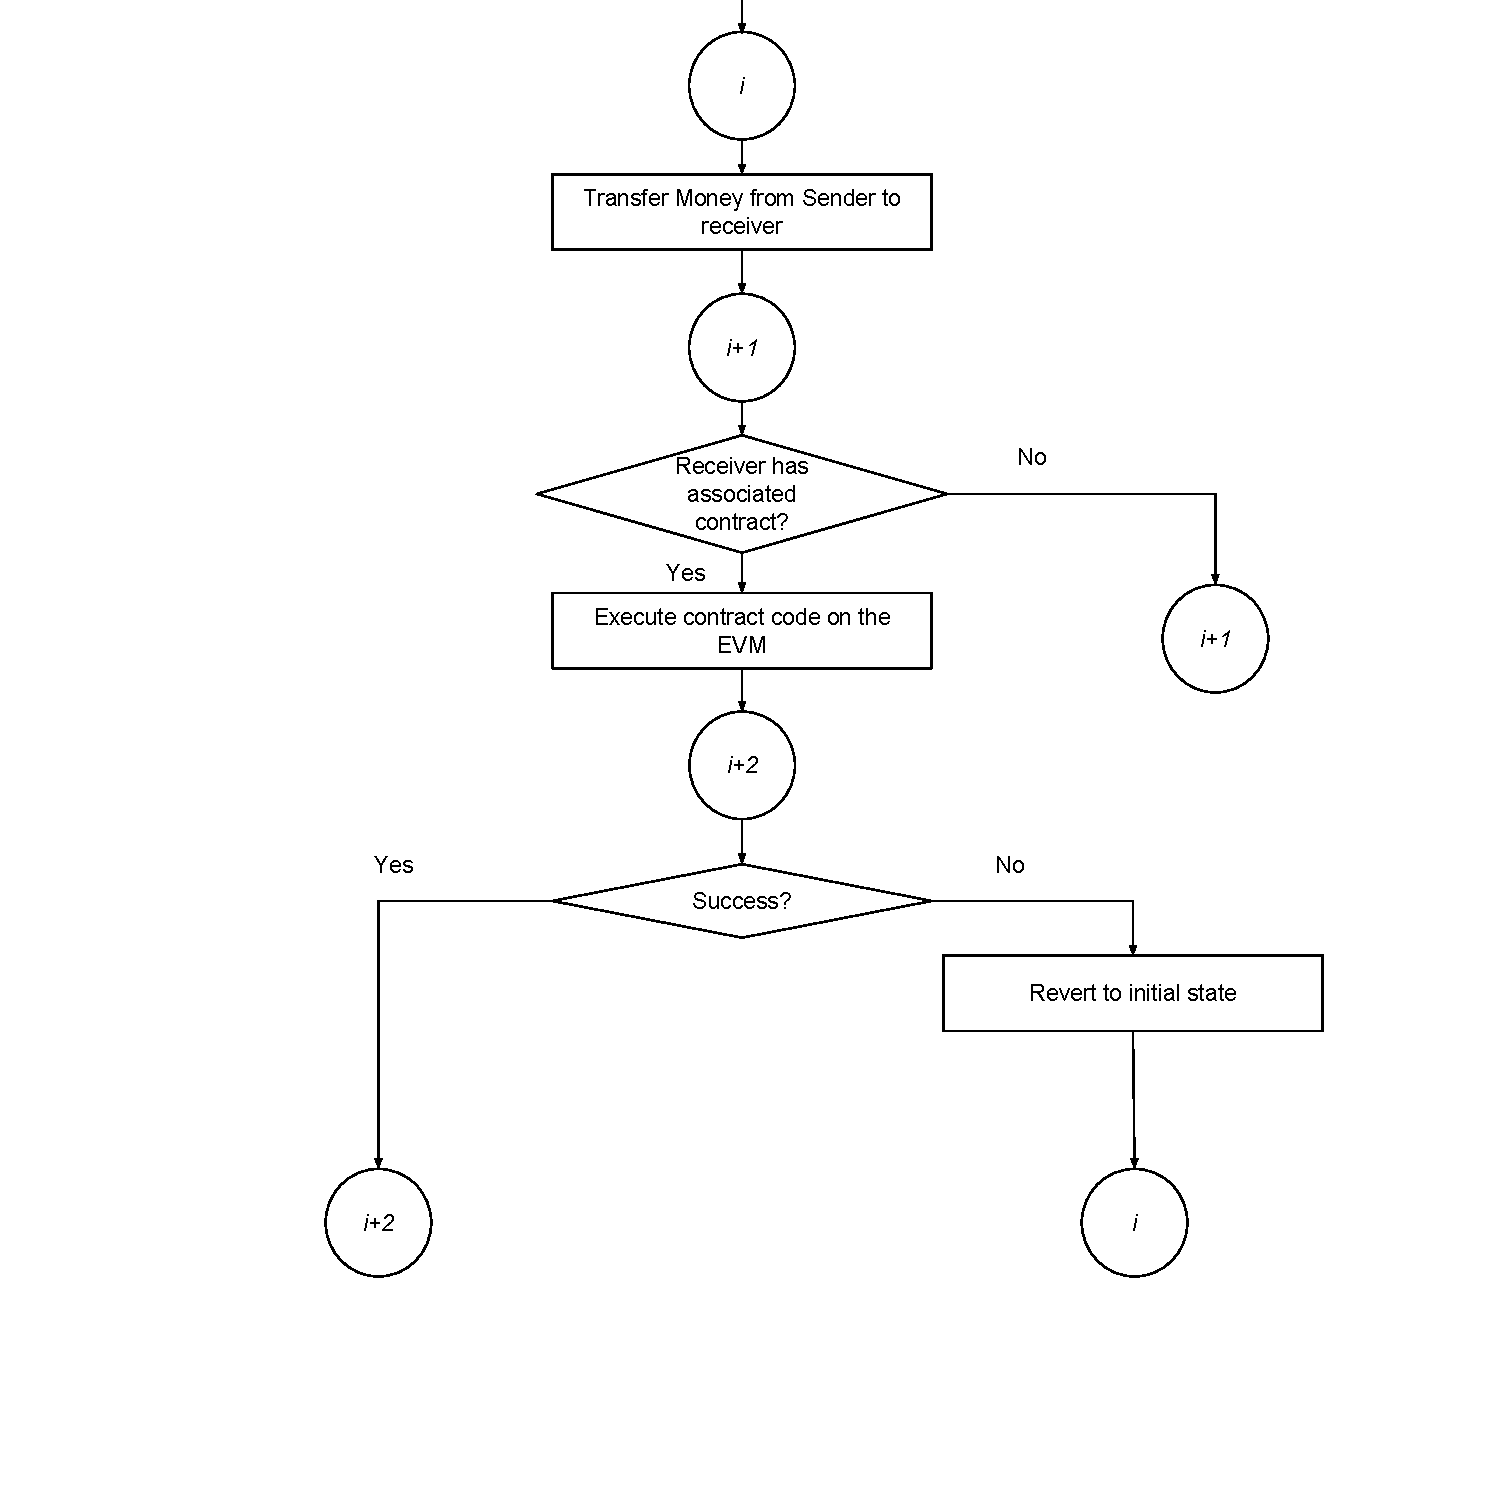
\includegraphics[width=\textwidth]{./res/img/message-call.pdf}
	\end{center}
	\caption{The steps of the message call execution algorithm.}
	\label{fig:message-call}
\end{figure}

The first step in the message call algorithm is the transfer of value from the
sender to the receiver account. If the recipient of the message is an externally
owned account, the message call terminates, otherwise the contract of the
account is executed on the EVM. If during this execution an error occurred (e.g.
stack overflow/underflow, out of gas exception), the used gas is not refunded
and the state is reverted to the state prior to the execution. This means that
the sender looses the gas but recovers the sent value. If the execution succeed,
this state persists. The steps of the algorithm are illustrated in
\autoref{fig:message-call}.